% -- Implementation ---------------------------------------

\section{Implementation}

The approach described in the previous section wasn't implemented in a day, obviously. This section will cover some difficulties that came along during the lab.

\subsection{The Fix}

Halfway the lab, a fix was introduced to take care of the stride issue. The stride values were now set and did not have to be passed on using \mcode{\_\_DATA\_START}. In order to make the $\rho$-VEX read the pixels in the data memory correct a pointer to the first address would be enough.

Unfortunately, this caused us problems for weeks. Since we wanted to let the original x264 file unaltered, we copied the folder and created a new application. The folder was called 'lab2', with the \mcode{pixel.c} file called \mcode{microlab2.c}. The \mcode{lab2.c} file containing the extracted kernel was in the rovex-examples folder because of the \mcode{makefile}, that was also residing there. Now, the fix was only applicable to the original x264 folder, so we still had to deal with the stride issue.

When we found out about this fix, we adjusted the original x264 folder. We commented out the source code of \mcode{pixel_satd_8x4} and put our MicroBlaze kernel code instead. To check whether the pixels were sent to $\rho$-VEX data memory correctly, we pre-defined two pixels in \mcode{pixel.c} to be written to \mcode{rvex-dmemory}. This way, we could have certain expectations when doing a \mcode{hexdump} to examine the registers. Our testpixels are shows in figure \ref{fig:test}.

\begin{figure}
	\centering
	\begin{subfigure} [h] {0.5\textwidth}
		\centering
		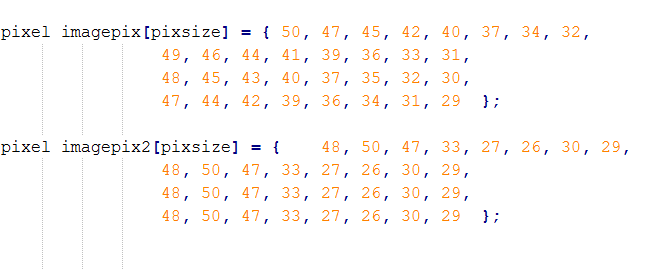
\includegraphics[width=150px]{Pictures/testpixels}
		\caption{Test pixels defined in \mcode{pixel.c}}
		\label{fig:test}
	\end{subfigure}
	\quad
	\begin{subfigure} [h] {0.5\textwidth}
		\centering
		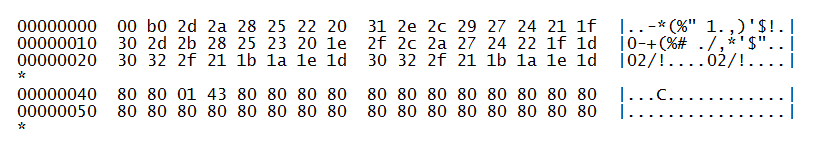
\includegraphics[width=150px]{Pictures/hextest}
		\caption{Hexdump of the testpixels (first two bytes incorrect)}
		\label{fig:testhex}
	\end{subfigure}
	\quad
\caption{Commands for reading from and writing to the $\rho$-VEX}%
\label{}%
\end{figure}


\subsection{Order of Variable Initialization}

After moving our code to the original x264 code and creating test pixels to be used for SATD calculation, a dump of the $\rho$-VEX data memory can been seen in figure \ref{fig:testhex}. As you can see, the first two byte are not matching. At first, we thought this could be because of the fact that another group was running their application at the same FPGA concurrently. However, the value of these bytes remained the same during several runs. 

This unwanted write was caused by the initialization of the \mcode{sum} variable, that has type \mcode{short int} and was stored in the data memory before the pixel. When \mcode{pixel_satd_8x4} tried to find the pixels, it found \mcode{sum} instead of the pixels, causing the program to get stuck in a loop. When changes \mcode{sum} to not being initiazlied, \mcode{datamem} containing the pixels had the first spot at address 120.

\subsection{Endianness}
*** byteswap toelichten ***